\documentclass{jsarticle}
\usepackage[dvipdfmx]{graphicx}

\title{楽しい運動計測実習に関するレポート}
\date{\today}
\author{奥屋 直己}

\usepackage[height=26cm,width=16cm]{geometry}

\graphicspath{{./images/}}

\begin{document}

\maketitle

\section{実験の目的}

腕をゆっくり動かすときや速く動かすとき、筋肉はそれに伴って強さを変化させる。しかし、それだけで速度が変えれるのだろうか。また、ゆっくり動かそうとするときに、力を加え続けてしまうと、腕は加速してしまう。では、どのようにして筋肉は速度を制御しているのだろうか。本レポートでは、腕を伸ばす、曲げるの繰り返し運動を行うことで、この理由を明らかにすることを目的とした。

\section{手法}

\subsection{実験}

今実験は右腕を水平面内で伸ばす、曲げるの繰り返し運動を行い、手首、肘、肩の3点の軌道と筋電の波形を計測した。被験者には指示せずに動かしやすい速度で動かす場合と、それよりも速く動かす場合の2つを指示した。3点の軌道の計測は、それぞれに反射マーカーをつけ、真上に設置した高速度カメラを使った。筋電の計測は、上腕二頭筋と上腕三頭筋に筋電計用電極を取り付け計測した。
それぞれ、サンプリング周波数は筋電が200 [Hz]、軌道を1000 [fps]とし、同時パルス発生装置を使い、開始時刻を同期した上で20秒間計測した。この実験では2人の被験者で行った。ただし、1人はデータがうまく取れなかったため、データは実質1人分となった。
\subsection{解析}

今回は筋電センサ(LOGICAL PRODUCT:ワイヤレス筋電センサ乾式)による筋電データとモーションキャプチャ(Library:Move-tr/3D)による運動軌道データを別々のプログラムで作成する。

\subsubsection{筋電データ}

筋電データには計測したデータの他にノイズが混ざっていると予測されるため、データの1~40Hzに対してバンドパスフィルタ(3次バターワークス)をかけることにより、低周波のノイズを除去した。また、単純にバンドパスフィルタをかけるとデータのピーク位置が実際のデータよりもすこしおそくなってしまう。そのためpythonのfiltfilt関数を使うことにより、順方向と逆方向の両方から1回ずつフィルタをかけ、ズレをなくした。

次にC言語で筋肉の活動度a(t)を以下の式で評価した。

\begin{equation}
a(t)=\frac{1}{\Delta{T}}\int^{t+\Delta{T}/2}_{t-\Delta{T}/2} |E(t)|dt
\end{equation}

E(t)は筋電位、tはフレーム数、幅$\Delta{T}$の窓を200 [frame]とした。サンプリングは1000 [fps]なので、$t\pm\Delta{T}/2$より、$\pm0.1$ [s]間での筋電位の上昇度を算出することができた。

\section{結果}

図\ref{fig:motion1}が指示していない速さでの腕の軌道、図\ref{fig:motion2}が速く動かす時の腕の軌道である。この2つの図を比較すると、図\ref{fig:motion2}が速さが速い分、線の密度とブレは大きくなるが、軌道に大きな差がない。このことから、それぞれの筋電位に軌道の違いでの影響はなく、速さ変化のみに影響を受ける。図\ref{fig:EMG1}を見ると、上腕二頭筋の筋電位の山と、上腕三頭筋の筋電位の山がほぼ同じ所で発生していることがわかる。しかし、図\ref{fig:EMG2}を見ると少しわかりづらいが、上腕二頭筋の筋電位が山のとき、上腕三頭筋は谷になっており、指示していない速さの時と上腕三頭筋の山と谷が逆となっている。図\ref{fig:EMG1}をみると上腕二頭筋の筋電にはおよそ 0.005〜0.09 [mV]、上腕三頭筋はおよそ 0.01〜0.03 [mV]、図\ref{fig:EMG2}をみると上腕二頭筋は 0.06〜0.14 [mV]、上腕三頭筋は 0.04〜0.09 [mV]となり、上腕二頭筋と上腕三頭筋の筋電には両方とも速く動かしたほうが大きくなっている。

\begin{figure}[htbp]
  \begin{minipage}{0.5\hsize}
    \begin{center}
      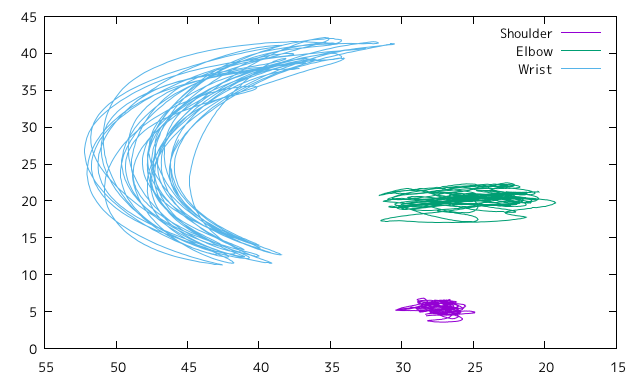
\includegraphics[clip,width=80mm]{Graph_2.png}
      \caption{指示していない速さでの運動での手首、肘、肩の3点の軌道(青=手首の軌道,緑=肘の軌道,紫=肩の軌道)。肘と肩はほぼ一定の位置で手首の軌道のみ大きく動いており、指示通りに腕を動かせていることがわかる。\label{fig:motion1}}
    \end{center}
  \end{minipage}
  \begin{minipage}{0.5\hsize}
    \begin{center}
      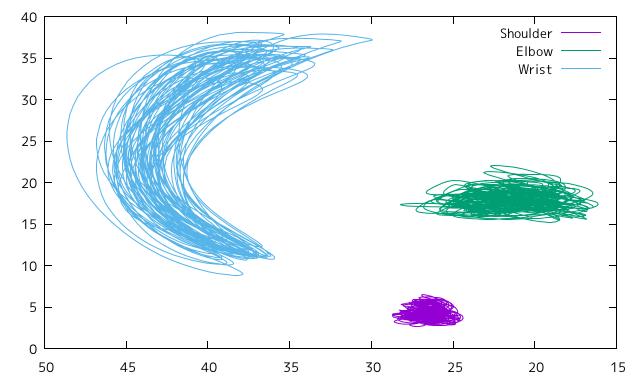
\includegraphics[clip,width=80mm]{Graph_3.png}
      \caption{図\ref{fig:motion1}よりも速く動かすように指示した場合の手首、肘、肩の3点の軌道(青=手首の軌道,緑=肘の軌道,紫=肩の軌道)。 図\ref{fig:motion1}と同様に手首のみが大きく動いており、指示通りに動かせていることがわかる。\label{fig:motion2}}
    \end{center}
  \end{minipage}
\end{figure}

\begin{figure}[htbp]
  \begin{minipage}{0.5\hsize}
    \begin{center}
      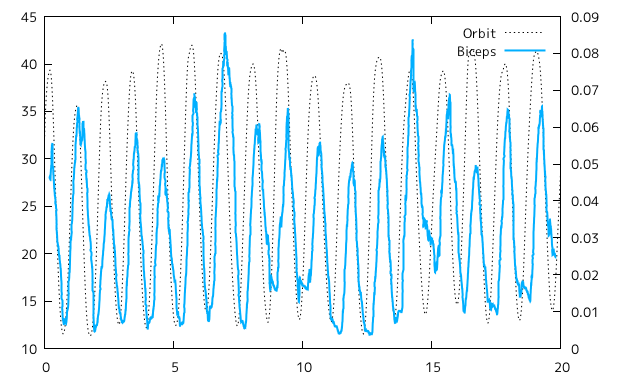
\includegraphics[clip,width=80mm]{Graph_4.png}
      \caption{指示していない速さで運動した時の上腕二頭筋と上腕三頭筋の筋電位(上腕二頭筋=青,上腕三頭筋=緑)。どちらの筋電にも腕の運動に合わせて振動している。 \label{fig:EMG1}}
    \end{center}
  \end{minipage}
  \begin{minipage}{0.5\hsize}
    \begin{center}
      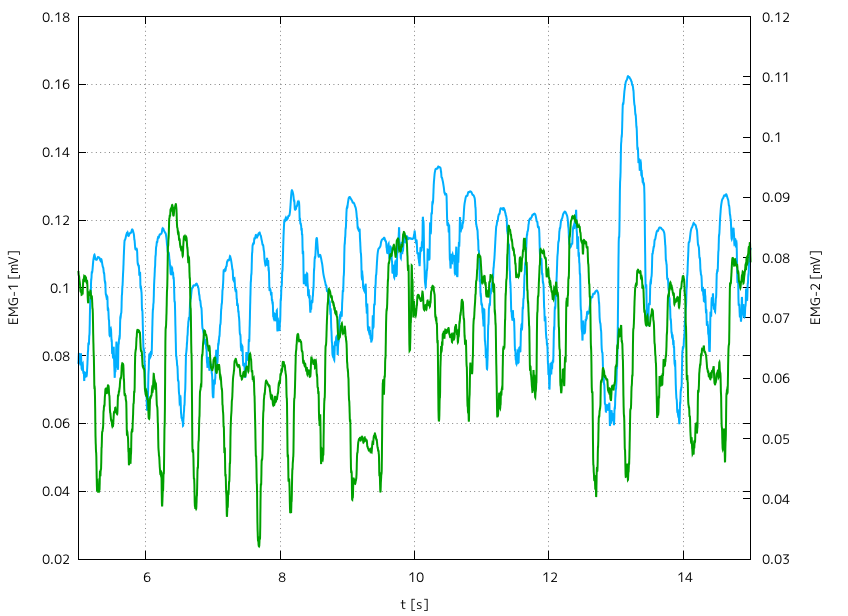
\includegraphics[clip,width=80mm]{Graph_5.png}
      \caption{速く動かす運動をした時の上腕二頭筋と上腕三頭筋の筋電位(上腕二頭筋=青,上腕三頭筋=緑)。左側のY軸が上腕二頭筋、右側のY軸が上腕三頭筋の筋電位を表す。 どちらの筋電にも腕の運動に合わせて振動している。\label{fig:EMG2}}
    \end{center}
  \end{minipage}
\end{figure}
  
\section{考察}
結果から指示していない速さのとき、上腕二頭筋と上腕三頭筋の筋電位の山がほぼ同じところで発生している(図\ref{fig:motion1})。また、上腕二頭筋は腕を曲げるために、上腕三頭筋は腕を伸ばすために使う筋肉である。更に、図\ref{fig:+length}から腕を縮めようとするタイミングで上腕二頭筋と上腕三頭筋の筋電位が山となっていることから、縮めようとするときに上腕三頭筋が逆方向に力を及ぼし、ブレーキのようになっていることがわかる。逆に、速く動かした時では、結果から、上腕三頭筋の筋電位の山と谷が逆になっていた。この場合、上腕三頭筋は腕を曲げるときにほぼ筋力は働いていない。また、結果より、上腕二頭筋と上腕三頭筋の筋電には両方とも速く動かしたほうが大きくなることもわかった。これらより、腕をゆっくり動かす場合と速く動かす場合の違いは、伸ばす時、または曲げる時の筋力の大きさもあるが、ブレーキの有無による違いも大きく関わるのではないかと考える。

\begin{figure}[htbp]
  \begin{center}
    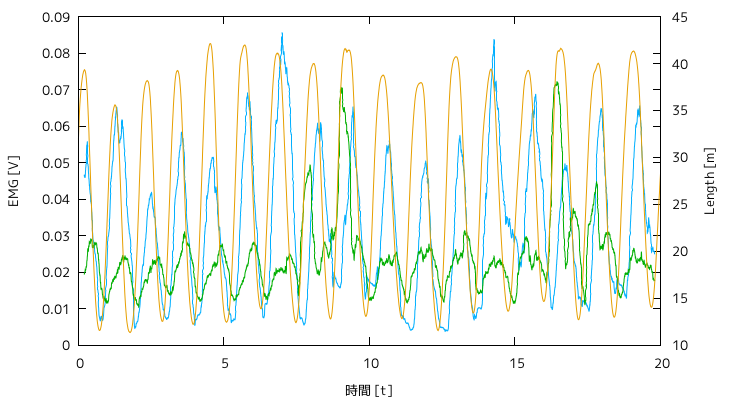
\includegraphics[clip,width=120mm]{Graph_6.png}
    \caption{図\ref{fig:EMG1}に図\ref{fig:motion1}から手首の運動軌道のY軸を重ねた図。左Y軸が筋電位(上腕二頭筋=青,上腕三頭筋=緑)、右Y軸が手首の移動距離(=黄色)となっている。手首の軌道は山の時、腕は伸びており、谷の時、腕は曲がっている。\label{fig:+length}}
  \end{center}
\end{figure}
\end{document}